\relatorio
{Crescimento da população em situação de rua e a capacidade de atendimento dos Centros POP em 2021 no município de São Paulo: um estudo descritivo. }
{
    \noindent Políticas Públicas

    \noindent Pesquisadores: Ana Beatriz Parra Ferreira, Arthur Sóter Assis, Giulia Beatriz Brombine Alves Rodrigues
    
    \noindent Orientadora: Laura Abreu
}
{
    O presente estudo investiga a capacidade de atendimento dos Centros POP em 2021 em relação ao crescimento da população em situação de rua em São Paulo nos últimos anos. Para isso, utilizam-se dados de Registros Mensais de Atendimentos (2017-2021) e Censos da população em situação de rua (2015-2021) a fim de se analisar a oferta e demanda desse equipamento de políticas públicas. A partir desse trabalho, é possível concluir que a capacidade de atendimento dos Centros POP não foi suficiente para suprir a demanda advinda do aumento significativo da população em situação de rua em São Paulo no ano de 2021.
}
{População em situação de rua, Centro POP}

\section{Introdução}

O Artigo 5 da Constituição Federal brasileira é frequentemente considerado a espinha dorsal dos direitos fundamentais e liberdades individuais do país. Este conjunto de princípios e garantias constitui a base para uma sociedade mais justa e igualitária, na qual os cidadãos devem gozar de proteção legal e respeito aos seus direitos. No entanto, existe uma parcela vulnerável da população que parece não gozar das mesmas garantias constitucionais, pois, enfrenta constantemente a violação flagrante de todos os direitos previstos pela Carta Magna. Trata-se da população em situação de rua.

Definida pelo Instituto Brasileiro de Geografia e Estatística (IBGE) como um “Grupo populacional heterogêneo constituído por pessoas que possuem em comum a garantia da sobrevivência por meio de atividades produtivas desenvolvidas nas ruas, os vínculos familiares interrompidos ou fragilizados e a não referência de moradia regular”, a população em situação de rua vivencia diariamente manifestações extremas da desigualdade e da vulnerabilidade social. Pessoas nessa condição enfrentam desafios diários para satisfazer necessidades básicas, como abrigo, alimentação, saúde e segurança  \cite{serafinocentro}. De modo síncrono, este grupo é regularmente vítima de discriminação, violência e negligência, tendo violados os seus direitos fundamentais, como a igualdade perante a lei, a integridade física e moral, a dignidade e a inviolabilidade da vida.

De tal modo, planos de ações e políticas públicas voltados a Pop. Rua são construídos e executados, com intuito de fornecer condições básicas de sobrevivência, como acesso a refeições, higiene, atividades de lazer e convivência, majoritariamente, por meio de um equipamento de assistência social. Em um estudo sobre a relação Estado - Pop. Rua brasileira, \cite{barbosa2018implementaccao} faz uso de fontes documentais e históricas para demonstrar como este segmento populacional foi inserido, apenas, em meados dos anos 2000 na agenda do governo federal no que se refere à estruturação de políticas públicas de inclusão e proteção social, divergindo das anteriores iniciativas de repressão e controle. De tal forma, verifica-se a importância de se compreender o funcionamento e estado atual das estratégias e equipamentos oferecidos à esta parcela, historicamente à margem das prioridades dos poderes públicos.

Consoante à esta realidade, este grupo sofreu um crescimento populacional expressivo nos últimos anos  \cite{silvaaumento}. Devido à falta de abundância em dados oficiais sobre a população nas ruas, modelos lineares são utilizados para estimar essas pessoas. Em pesquisas realizadas pelo Ipea, estima-se que a população brasileira em situação de rua era composta por aproximadamente 102 mil pessoas em 2015 \cite{natalino2016estimativa}. Em 2022, utilizando o mesmo modelo linear, a população em situação de rua era composta por aproximadamente 281,5 mil pessoas, de forma que em uma década o crescimento foi de 211\% .

Uma vez que o Brasil não conta com dados oficiais sobre a população em situação de rua, majoritariamente devido a dificuldade de obtenção de dados, e destacando como tal fato reproduz e invisibiliza socialmente a Pop. Rua no âmbito das políticas sociais, tornando marginal e ou inexistente o planejamento, a inclusão e o acolhimento destes, enfatiza-se a relevância do uso das informações disponíveis sobre a mesma em prol da produção de uma análise descritiva capaz de gerar evidências sobre as relações de oferta e demanda de equipamentos de assistências sociais que a atendem. 

A população em situação de rua se refere a um grupo cuja assistência social requer um equipamento de nível de média a alta complexidade. O principal equipamento para atender esse grupo é o Centro de Referência Especializado para População em Situação de Rua (Centro POP), ou, na ausência de uma unidade de Centro POP na região ou município, o Centro de Referência Especializado de Assistência Social (CREAS). Inicialmente, para a análise da cidade de São Paulo, as unidades do CREAS presentes nas zonas municipais que não contam com a presença de um Centro POP foram consideradas como objeto de estudo. Entretanto, após uma devida análise dos dados, utilizar o CREAS como ferramenta de pesquisa foi uma abordagem desconsiderada, assim como será detalhado na seção \ref{anades}. 

Desta maneira, o seguinte estudo teve como principal proposito desenvolver uma análise descritiva de Centros POP na cidade de São Paulo, examinando as relações de oferta e demanda dos atendimentos nas unidades presentes no município. 


\subsection{Centros POP}
Os Centros de Referência Especializado para População em Situação de Rua, popularmente conhecidos como Centros POP, representam um elemento fundamental na estrutura de políticas públicas voltadas para indivíduos em condições de vulnerabilidade. Estes centros são projetados para fornecer uma gama de serviços que vão além do atendimento das necessidades básicas, desempenhando um papel crucial na reintegração social e na garantia de direitos dessa população. O funcionamento das unidades é garantido a partir do aporte do Governo Federal, juntamente com estados e municípios.

Os serviços oferecidos pelos Centros POP incluem acesso a alimentação, higiene pessoal e fornecimento de roupas, essencial para a promoção da dignidade dessas pessoas. Além disso, o atendimento psicossocial oferecido nesses centros aborda questões de saúde mental e fornece suporte emocional, considerando os desafios únicos enfrentados por aqueles que vivem nas ruas. A assistência para regularização de documentação é outra funcionalidade de alta relevância, pois é um passo fundamental para o acesso a outros direitos e serviços públicos. Vale também destacar que os Centros POP realizam o encaminhamento dos indivíduos que atendem para serviços de saúde e oportunidades educacionais, além de promoverem atividades voltadas para a reintegração social e profissional, como oficinas, cursos e atividades culturais voltadas à Pop. Rua.

Nesse estudo, a escolha de focar nos Centros POP se deu pela sua relevância direta e significativa para a população em situação de rua. Isso porque estes centros não foram pensados apenas para atenderem às suas necessidades imediatas de subsistência, mas também para oferecerem atendimentos com profissionais de assistência social, psicologia, sociologia, terapia ocupacional entre outros, a fim de construir caminhos para a superação de seus desafios complexos diários.

Sendo assim, vale destacar que no município de São Paulo existem seis unidades desse equipamento em diferentes bairros:
\begin{enumerate}
    \item Centro POP BELA VISTA
    \item Centro POP SANTA CECÍLIA
    \item Centro POP MOOCA
    \item Centro POP VILA MARIA
    \item Centro POP SANTANA
    \item Centro POP SANTO AMARO
\end{enumerate}

Todas foram incluídas no estudo. De cada uma, analisou-se os registros mensais de atendimento (RMA's) e a quantidade de profissionais em seu quadro de colaboradores por profissão.

Por fim, vale dizer que os Centros POP representam um ponto de intersecção entre as necessidades imediatas da população em situação de rua e as políticas públicas destinadas a atendê-la. Ao analisar a relação de oferta e demanda desse equipamento, pode-se compreender de que maneira essa iniciativa governamental de fato chega "na ponta" e se a quantidade de atendimentos registrados variou tanto quanto os números de pop rua no ano de 2021 na cidade de são Paulo.

\section{Revisão Literária}

Por meio de entrevistas, \textcite{rauppvulnerab} demonstram, a prevalência da violência e da violação de direitos pela parcela entrevistada que correspondia à população em situação de rua. Esse dado deixa claro que o acesso à políticas públicas de qualidade são essenciais para a proteção e garantia de dignidade à Pop. Rua do município de São Paulo.

Em outro paper, \textcite{serafinocentro} discutem o fenômeno da maior concentração de população sem-abrigo nos centros dos municípios devido à presença de trabalhos informais que representam possibilidades de renda e à disponibilidade de infraestruturas urbanas, como praças, pontes e vias nas quais essa população pode estabelecer sua moradia improvisada.

Vale destacar que a regulamentação da população de rua no Brasil ocasionou, não apenas a criação de equipamentos públicos e planos de articulação de combate ao crescimento da população de rua, mas também trouxe-os a um maior nível de visibilidade política, o que, em tese garantiria a continuidade de programas como o Centro POP, além de ser apontado como um marco da cidadania por estudiosos do tema \cite{medeirosbenesse}.

Contudo, sabe-se que as políticas sociais não necessariamente atingem todos os objetivos para os quais foram elaboradas e, pensando nisso, este estudo foi norteado pela seguinte questão: A capacidade de atendimento dos Centros POP acompanhou a demanda crescente do município de São Paulo em 2021?. 

Vale destacar por fim, que parte da metodologia do presente artigo foi baseada no trabalho da Secretaria de Desenvolvimento Social da Criança e Juventude do Governo do Estado do Pernambuco (SDSCJ), principalmente porque os seus pesquisadores também realizaram o cruzamento entre a oferta dos serviços oferecidos pelos Centro POP dos municípios de Pernambuco e a demanda, representada pelo censo da população em situação de rua.  \cite{secretariaPernambuco}.

\section{Metodologia}

Dada a relevância dos Centros Pop enquanto equipamentos de assistência social voltado à população em situação de rua, é crucial que esse público tenha acesso aos atendimentos ofertados por esses centros a fim de ter assegurados alguns de seus direitos mais básicos como alimentação e regularização de documentos. Partindo desse ponto, esse trabalho buscou compreender a relação entre oferta e demanda por tais atendimentos nesses equipamentos.

Para isso, foram analisadas as bases de dados de Registros Mensais de Atendimentos dos Centros Pop dos anos de 2017 a 2021 - Dado considerado a oferta de atendimentos desse equipamento para fins desse estudo, além do Censo da população em situação de rua do município de São Paulo dos anos de 2015 a 2021 - Considerado a demanda total pelos serviços oferecidos pelo Centro Pop.

Vale destacar que a opção metodológica por esses dados para oferta e demanda se deram principalmente, porque o Censo se mostrou a melhor base para descrever a pop rua e seu crescimento dos últimos anos e, além disso, porque o Registro mensal de atendimentos já foi analisado em estudos de oferta e demanda de Centros Pop. \cite{secretariaPernambuco}.

Por fim, realizou-se uma comparação entre as taxas de crescimento tanto da oferta (RMA dos Centros Pop) quanto da demanda (Número de pessoas em situação de rua) a fim de compreender se a capacidade de atendimento do Centro POP acompanhou a demanda crescente do município de São Paulo no ano de 2021.

\section{Dados}

A escassez de dados  oficiais atualizados é uma realidade que permeia o cenário de estudos sobre a Pop. Rua, de forma que a disponibilidade de dados teve influência na extensão geográfica avaliada no estudo. De modo relacionado, o município de São Paulo possui a maior concentração de pessoas em situação de rua no país e dispõe uma quantidade de dados e detalhamentos sobre a Pop. Rua maior do que os outros distritos brasileiros. O setor de pesquisa de SPGEO é responsável pelo eixo da Vigilância Socioassistencial, produzindo análises das informações territorializadas sobre as situações de risco e vulnerabilidade. De tal forma, uma vez que censos e relatórios sobre a população em situação de rua são disponibilizados pela prefeitura de São Paulo, o acesso à tais bases de dados favoreceu uma análise em escala municipal. 

Analogamente, o mesmo fator influenciou a análise temporal do estudo. Para a população de São Paulo presente nas ruas, a disponibilidade de informações censitárias se limitam aos anos de dentro do período de 2015 até 2021, o ano do último censo publicado até o momento da pesquisa. 

Para o estudo, 2 principais fontes foram utilizadas: o Censo da População em situação de rua e o Censo SUAS. O primeiro é disponibilizado pela prefeitura de São Paulo, enquanto o Censo SUAS é um processo de monitoramento que coleta dados por meio de um formulário eletrônico preenchido pelas Secretarias e Conselhos de Assistência Social dos Estados e Municípios, sendo disponibilizado pela Secretária Nacional de Assistência Social (SNAS). 

As bases adquiridas por meio do Censo SUAS e utilizadas foram as bases de dados gerais sobre os RMAs (Registro Mensal de Atendimentos) e as bases de RH sobre as equipes que casa unidade de serviço compunha em seu respectivo ano. Igualmente, o acesso temporal dessas informações se limitou aos anos de 2017 até 2021. 

\section{Análise descritiva}\label{anades}

A medida inicial da análise foi entender as características principais da Pop. Rua presente no Censo de São Paulo. De tal forma, buscou-se compreender a maneira como essa população estava distribuída pelo município. Assim como demonstra a figura \ref{fig:distrib}, a Pop. Rua se concentra de forma expressiva no centro da cidade. Ulteriormente, buscou-se traçar os vínculos entre as localizações das 6 unidades de Centros POP com a distribuição geográfica da população em situação de rua. A partir da figura \ref{fig:sp}, percebe-se que 5 das unidades tem presença na região central da cidade, com concentrações a partir de mais de 200 pessoas por $km^2$. 

\begin{figure}
    \caption{Distribuição da população em situação de rua em São Paulo }
    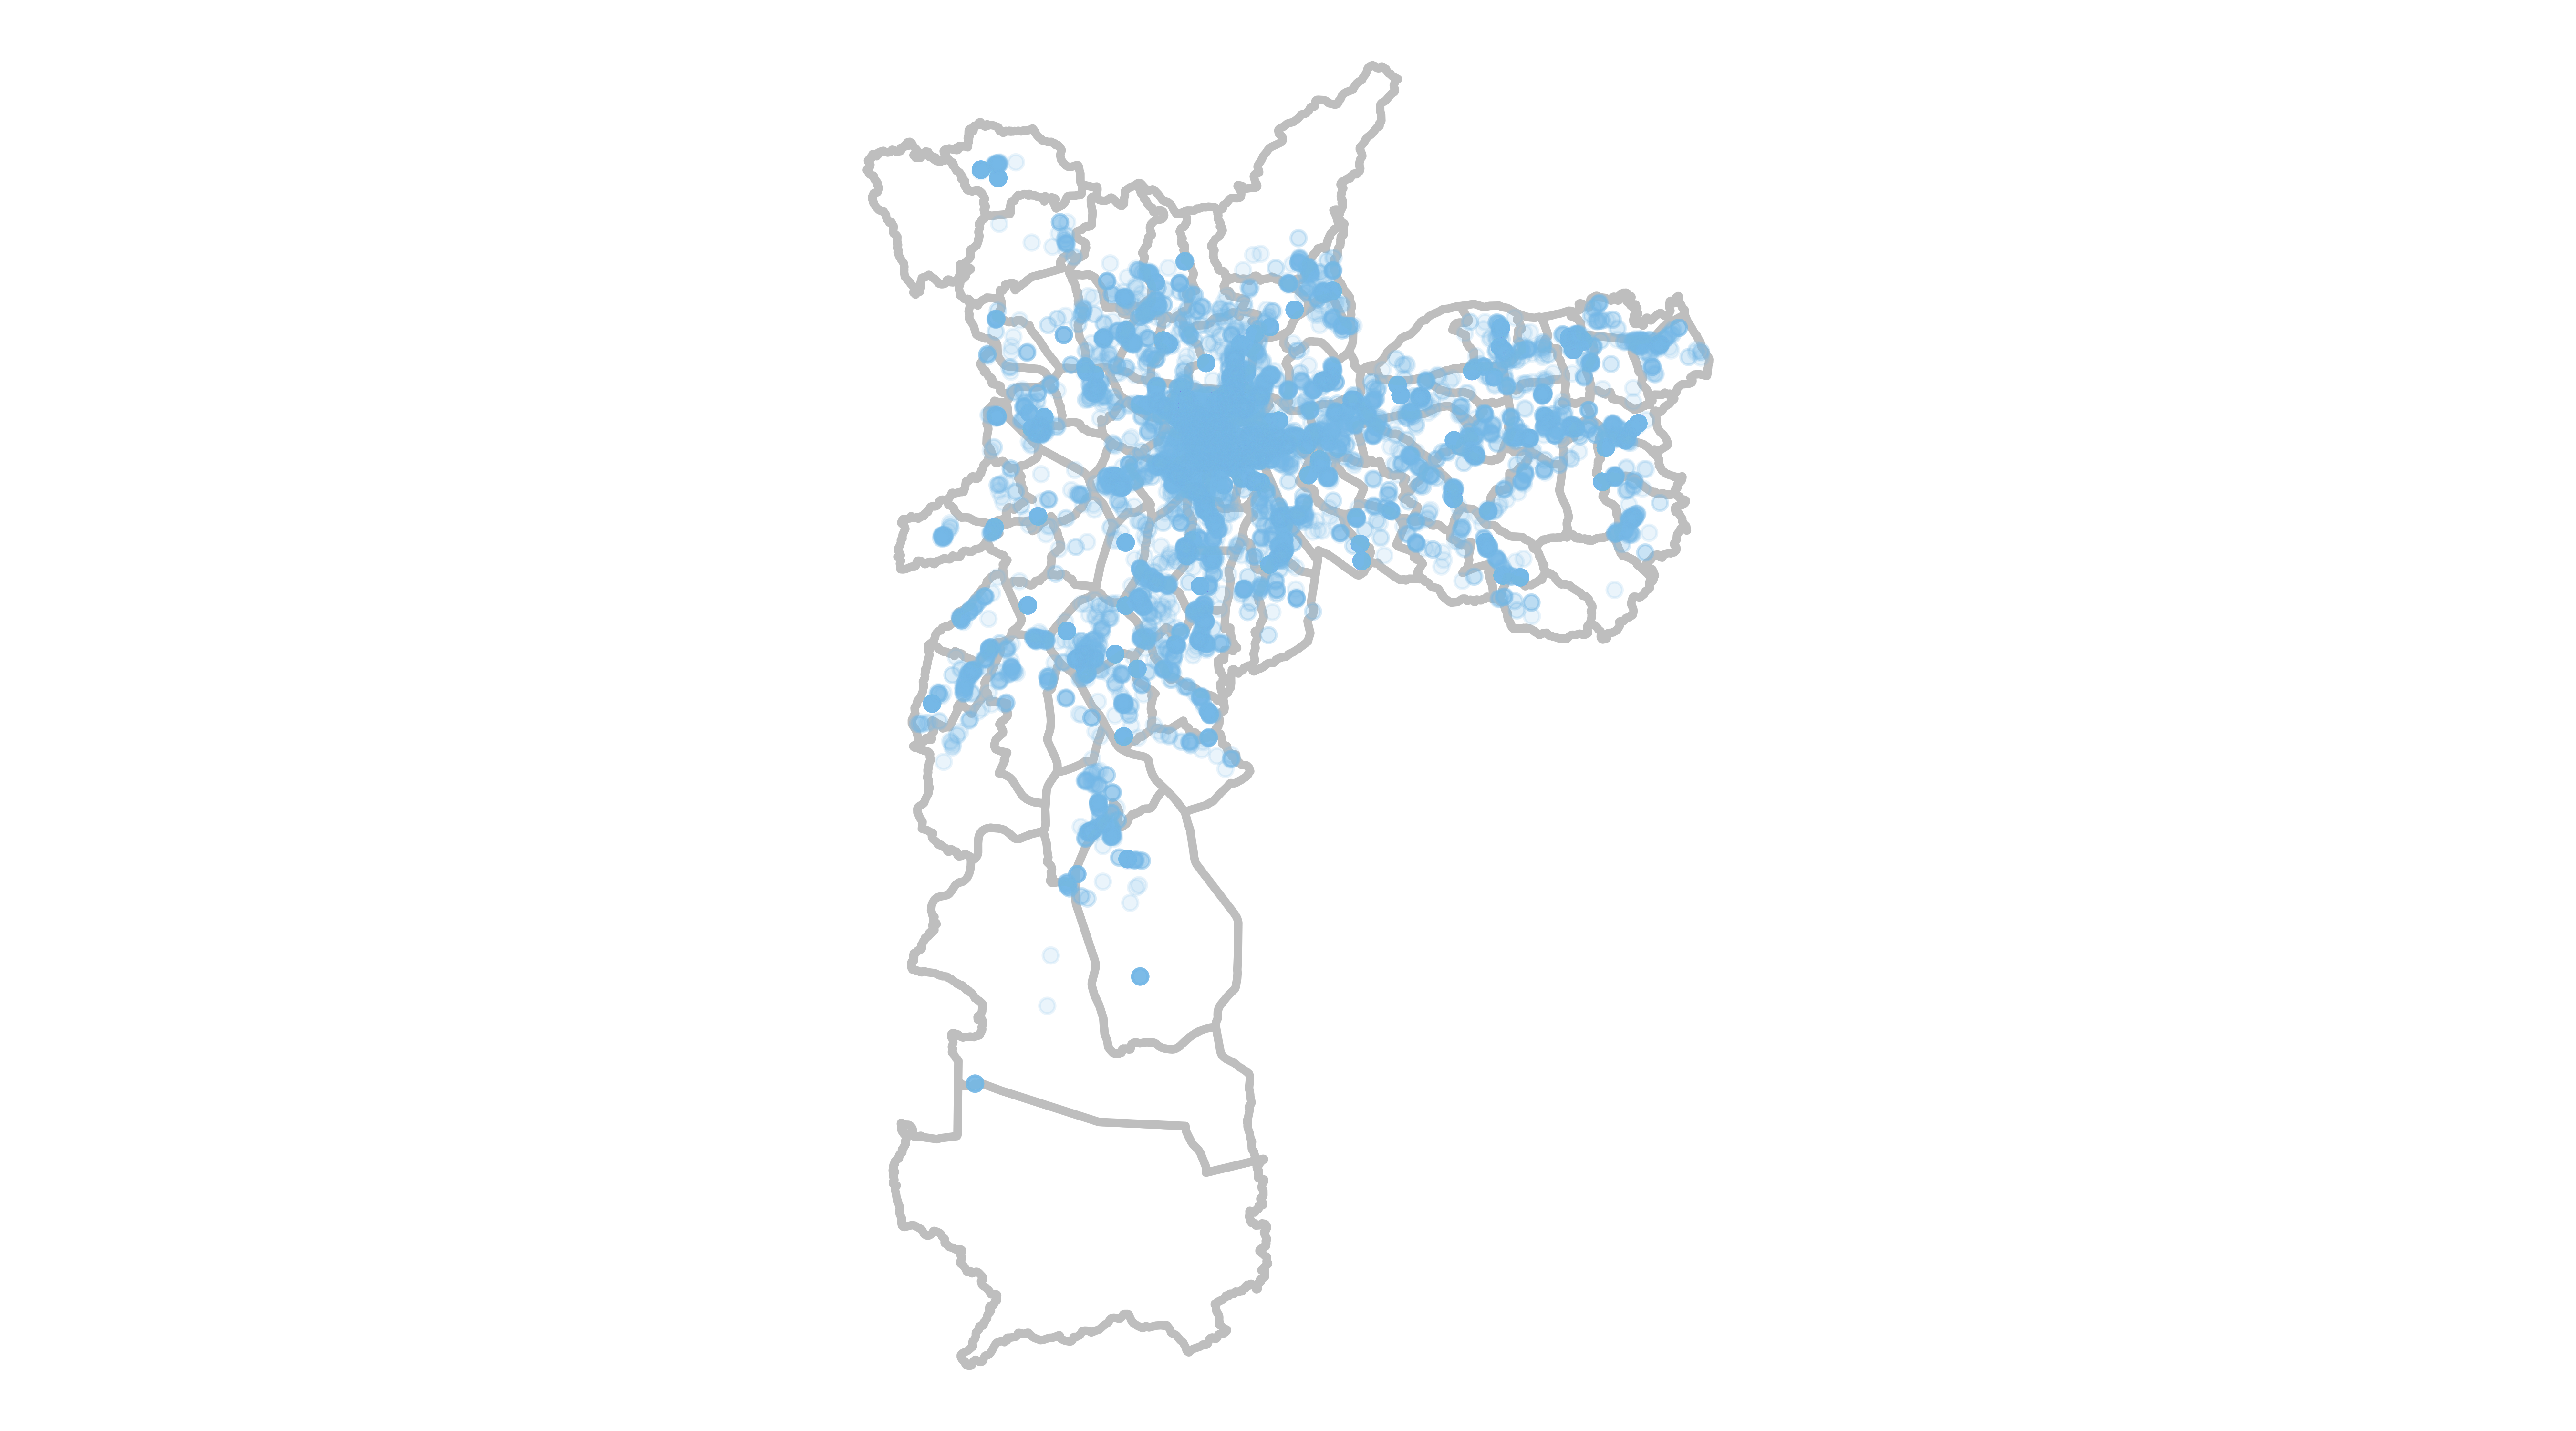
\includegraphics[width = .9\linewidth]{relatorios/grupo2/figuras/distribuicao.png}
    \label{fig:distrib}
\end{figure}
\begin{figure}
    \caption{Distribuição de Centros POP e População em situação de rua}
    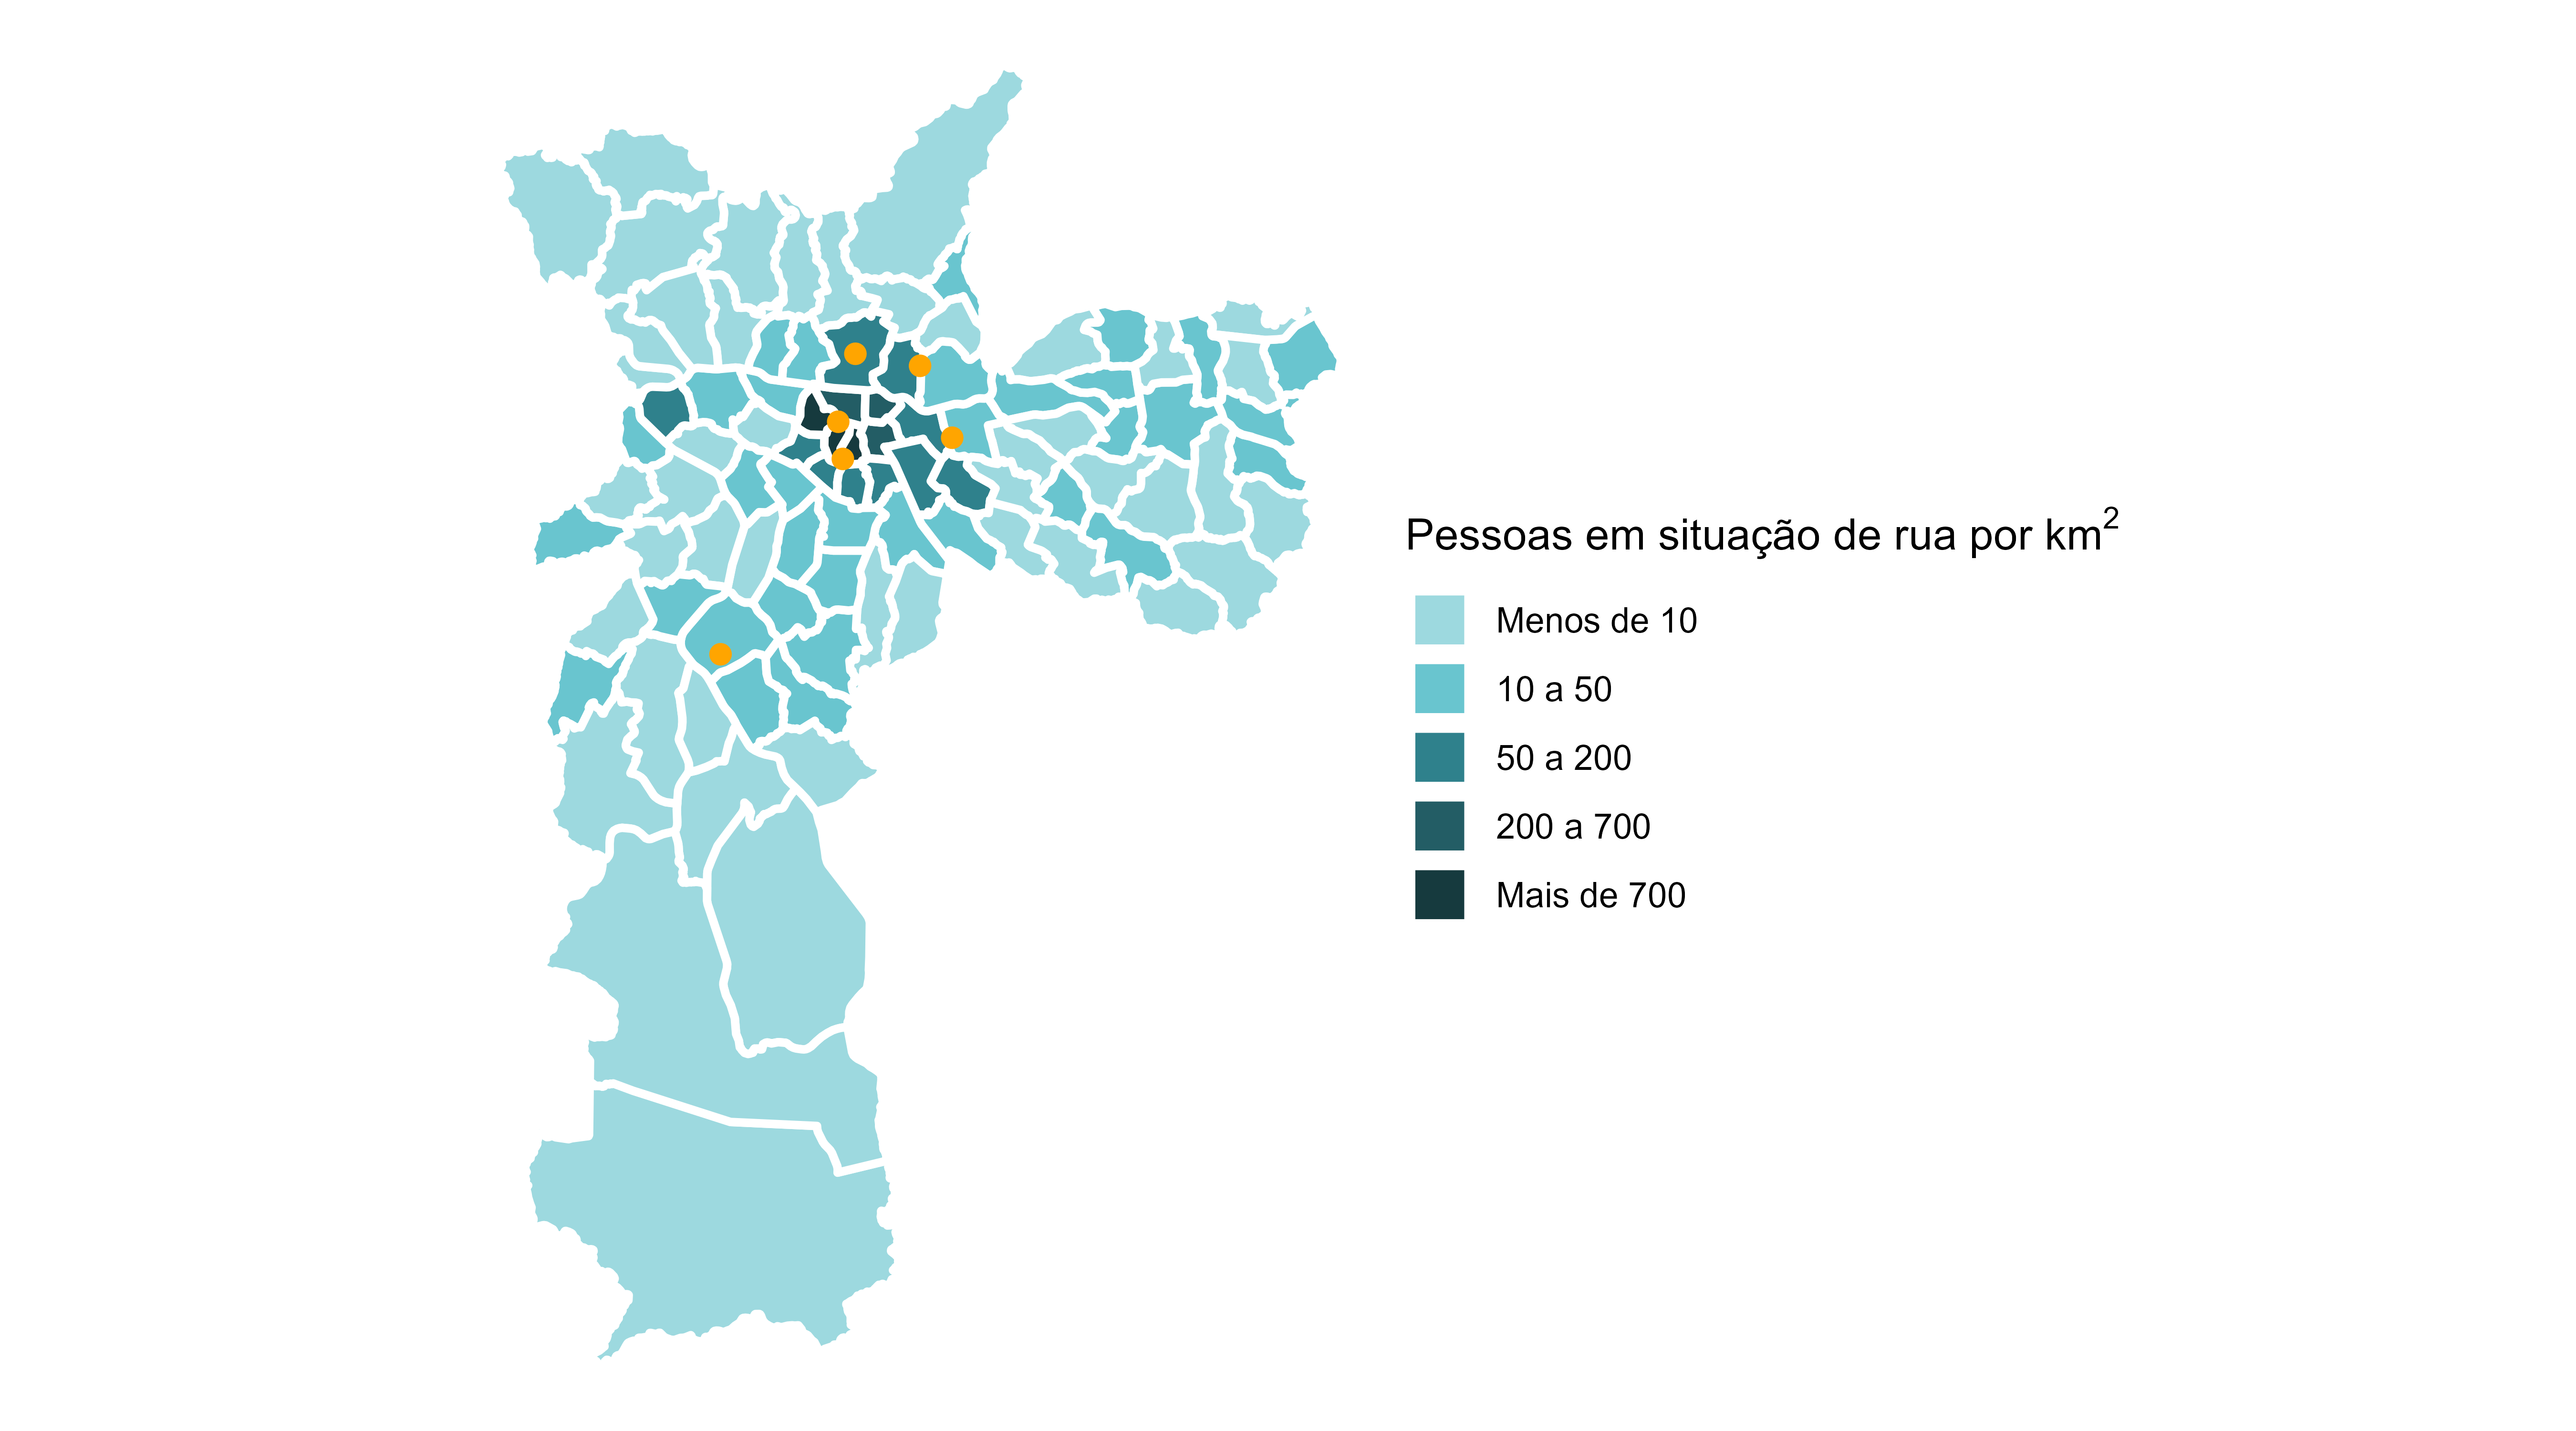
\includegraphics[width = .9\linewidth]{relatorios/grupo2/figuras/sp.png}
    \label{fig:sp}
\end{figure}

Inicialmente, considerou-se utilizar as informações de RMAs dos CREAS (Centro de Referência Especializado de Assistência Social) na zona oeste de São Paulo. A região se trata da única zona com ausência de unidades de Centro POP, de forma que, nestes casos, as unidades do CREAS passam a prestar determinados serviços a Pop.Rua, visando prevenir agravamentos das situações de risco pessoal 
e social. Vale ressaltar que o CREAS não funcionará como substitutivo do trabalho social desenvolvido no Centro POP, mas poderá ofertar acompanhamento especializado, na localidade, às essas pessoas em situação de rua, possibilitando a construção do processo de saída das ruas. 

De tal forma, incluir as unidades CREAS Pinheiros e CREAS Butatã foi uma abordagem para avaliar a capacidade de atendimento. Todavia, ao analisar os dados de atendimentos direcionados à população em situação de rua nestas unidades, viu-se que estas unidades apresentaram uma quantidade de atendimentos muito pequena para a Pop. Rua, assim como a tabela     \ref{tabelacreas} apresenta. Sendo assim, as duas unidades não foram mais incluídas em análises futuras. 

\begin{table}[h]
    \label{tabelacreas}
    \centering
    \begin{center}
        \caption{Nome}
            \begin{tabular}{||c c c||} 
            \hline
            Unidade do CREAS & Atendimentos totais & Atendimentos à Pop. Rua \\
            [0.5ex] 
            \hline\hline
            Pinheiros & 74 & 0  \\ 
            \hline
            Butantã & 655 & 10 \\ 
            
            \hline
        \end{tabular}
        \end{center}
\end{table}

% [1ex]

 hipótese de uma determinada relação entre profissionais, índice de recurso como oferta, e atendimentos foi avaliada a partir das taxas de variação dos mesmos. Examinando, portanto, a variação anual total de profissionais, apresentada na figura \ref{fig:variprof}, e comparando-a com a variação anual de atendimentos nos Centro POP, figura \ref{fig:variatend}, verifica-se que a quantidade de registros mensais apresenta semelhança no comportamento de variação com a quantidade de pessoas trabalhando na unidade de assistência social. De tal forma, parece existir uma alta correlação entre os dois. 

\begin{figure}
    \centering
    \caption{Variação anual do total de profissionais}
    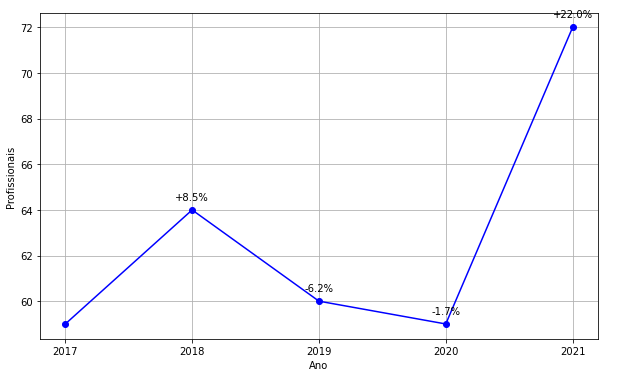
\includegraphics[width = .9\linewidth]{relatorios/grupo2/figuras/variacaoanualprof.png}
    \label{fig:variprof}
\end{figure}

\begin{figure}
    \centering
    \caption{Variação anual de atendimentos}
    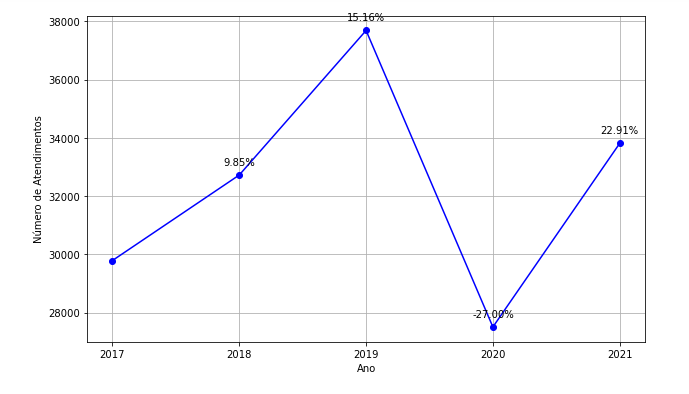
\includegraphics[width = .9\linewidth]{relatorios/grupo2/figuras/variacaoanualatendimentos.png}
    \label{fig:variatend}
\end{figure}

Por fim, analisando os valores absolutos de crescimento da população em situação de rua com os registros mensais de atendimento, a figura \ref{fig:variacao} demonstra as relações entre as duas variáveis.
Para a construção do gráfico, escolheu-se o início da pandemia de Covid-19 como a data designada como valor de referência, devido ao seu impacto na aceleração do crescimento da Pop. Rua. Logo, outubro de 2019 atua como referência (100), de modo que as variáveis População em situação de rua e Registro Mensal de Atendimento se localizam no mesmo ponto. Sendo este valor estabelecido, cada ponto no gráfico representa um comportamento proporcional à esta referência. Por exemplo, estando estabelecido que em 2019 houveram 100 atendimentos anuais, caso em 2021 a variável que representa Pop.Rua esteja acima de RMA, sabe-se que houveram menos do que 100 atendimentos, uma vez que a população aumentou mais do que o número de atendimentos.  

\begin{figure}
    \centering
    \caption{Variação cumulativa da população em situação de rua e RMA}
    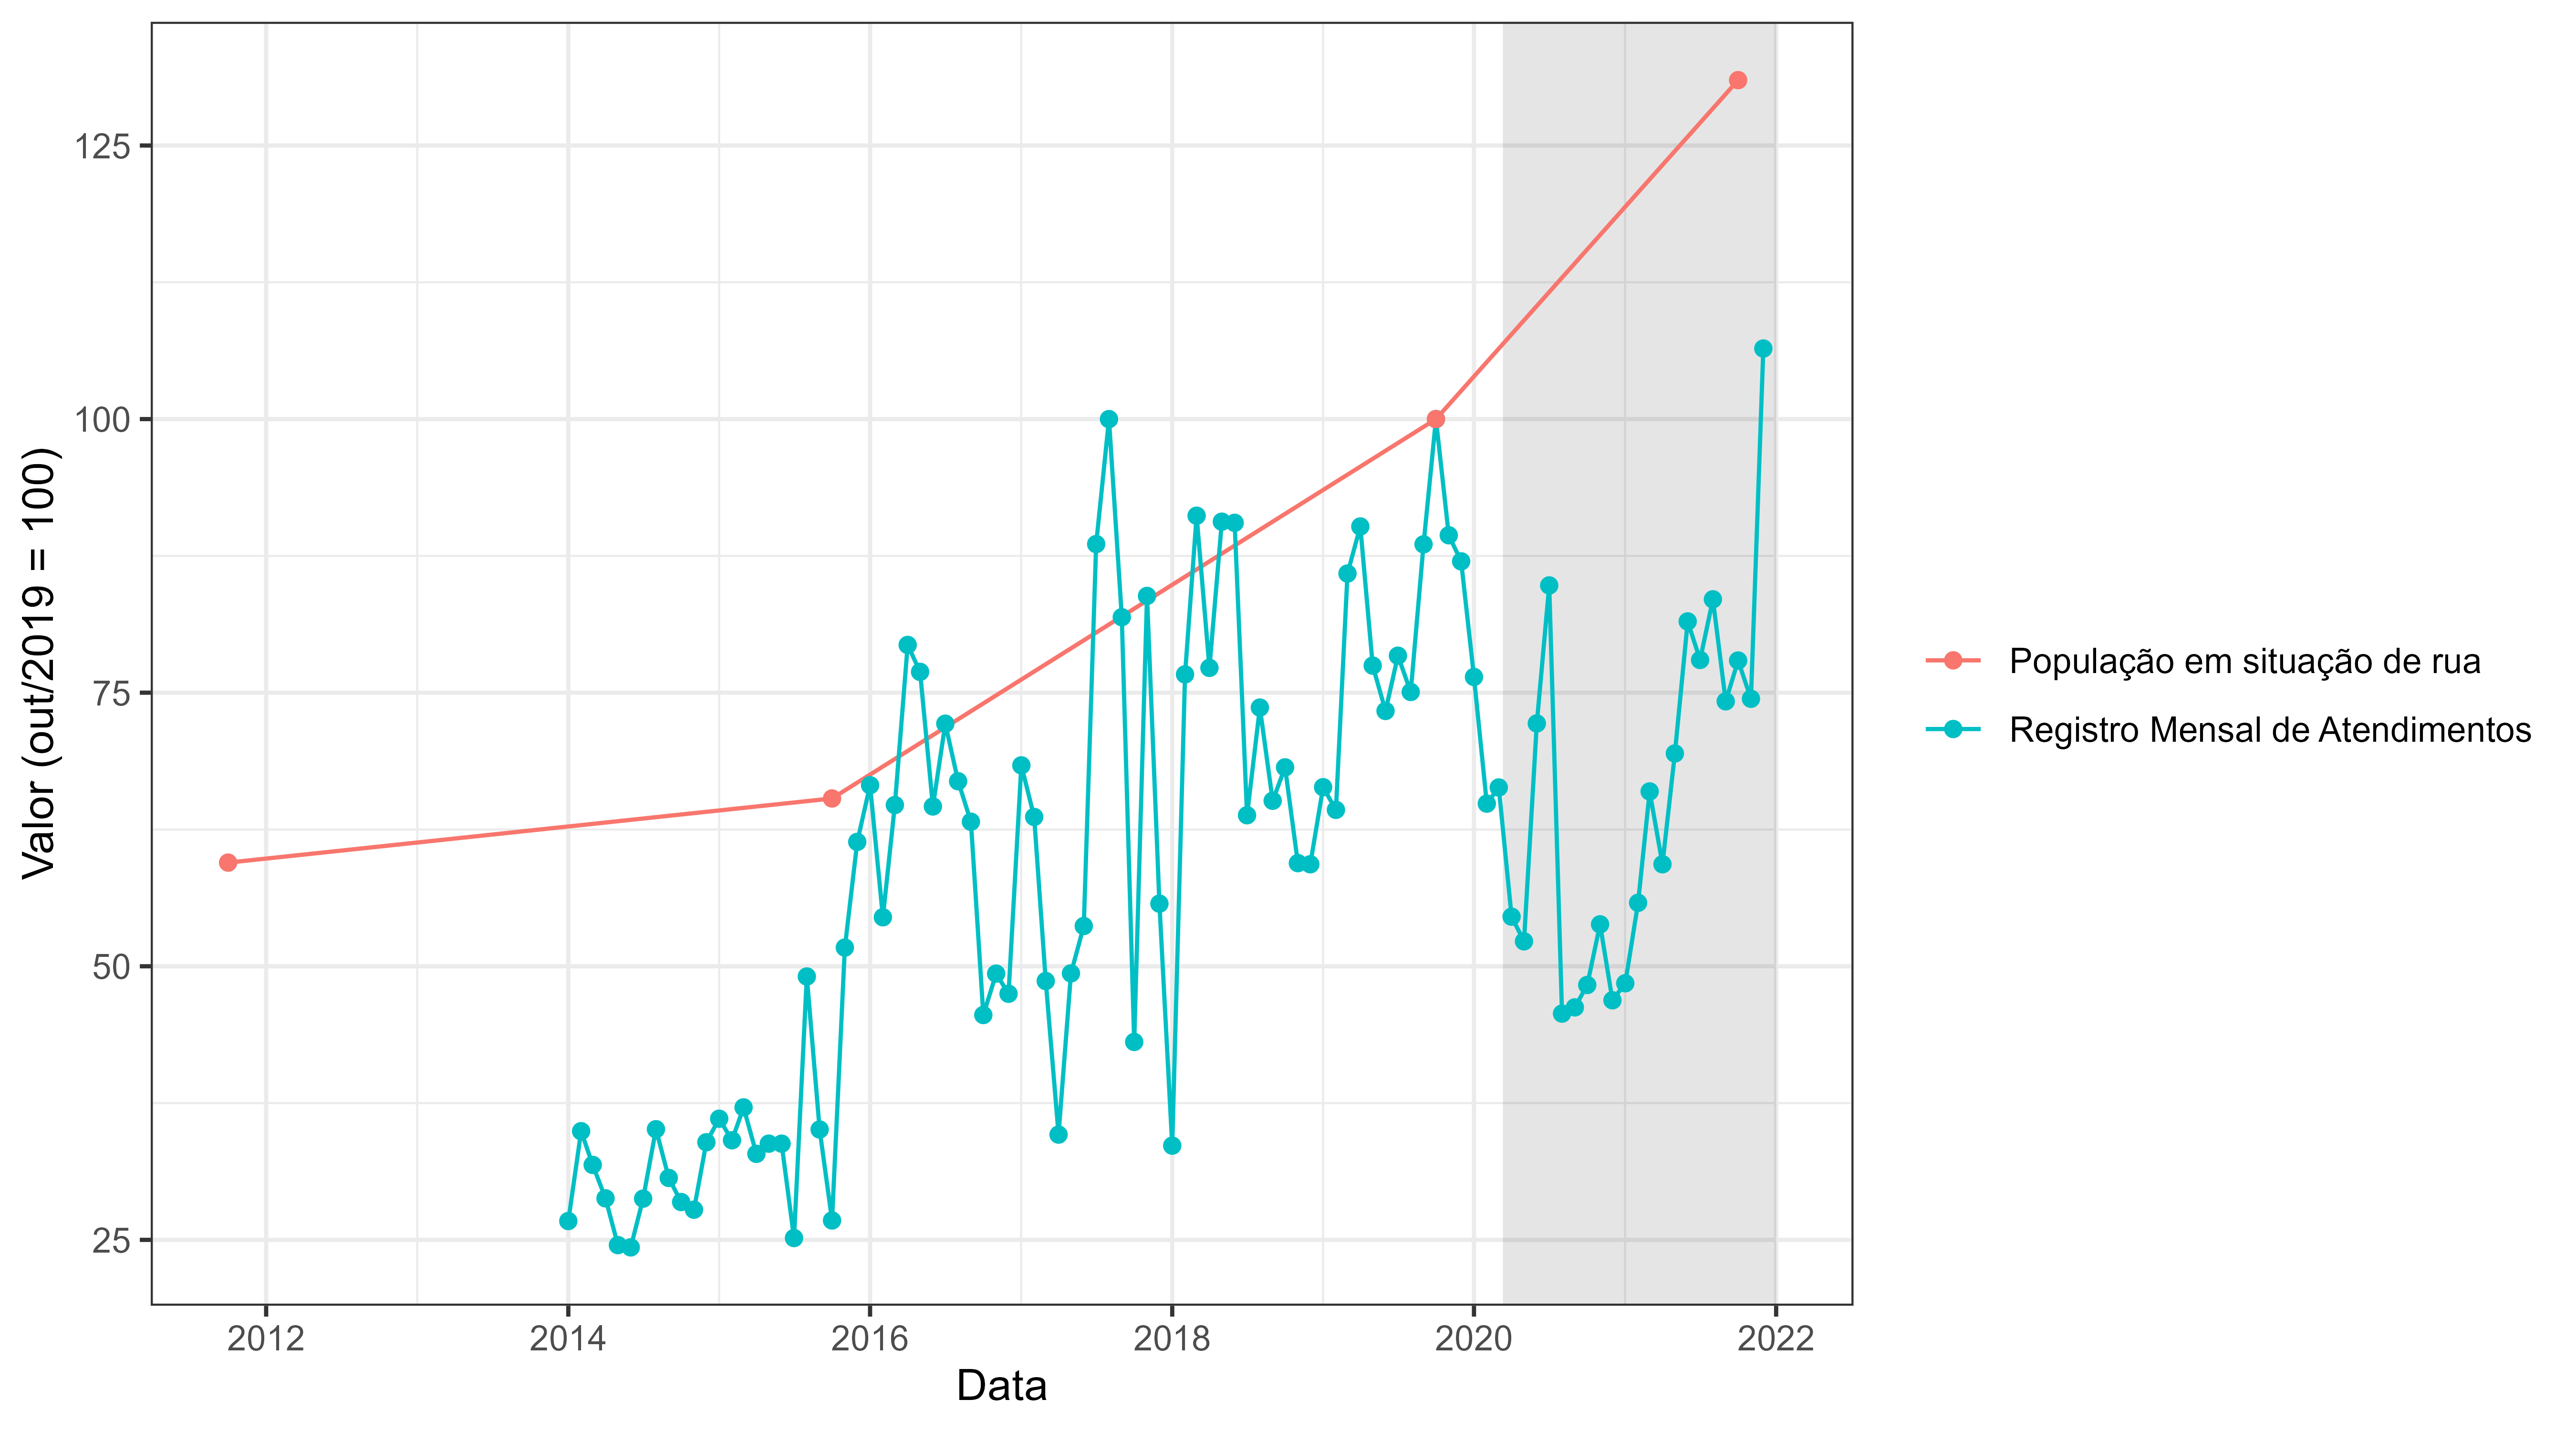
\includegraphics[width = .9\linewidth]{relatorios/grupo2/figuras/variacao.png}
    \label{fig:variacao}
\end{figure}

\section{Conclusões e limitações}

A partir das análises realizadas neste estudo, é possível afirmar que o a população em situação de rua  questão cresceu mais do que o número de atendimentos dos Centros Pop no município de São Paulo em 2021. Além disso, de acordo com os dados, cada pessoa em situação de rua foi atendida em média 1 vez por um Centro Pop ao longo de todo o ano de 2021.

Esse número é alarmante, porque significa que, em média, uma pessoa sem-abrigo acessa alimentação, banho e acolhida noturna uma vez a cada 365 dias em um Centro Pop. Partindo desse ponto, pode-se dizer que existem meios alternativos utilizados pela Pop. Rua para acessar seus direitos básicos, meios como o trabalho de organizações da sociedade civil e comunidades solidárias organizadas pela própria população sem-abrigo, que, apesar da relevância social, não oferecem estabilidade e capacidade de atender todos os que precisam, o que significa mais insegurança para uma população tão vulnerável.

Vale destacar ainda, que o apoio à Pop. Rua tem muitos obstáculos e dentre eles, destaca-se a lacuna nos dados estatísticos que fomentam as políticas públicas como os Centros Pop, dificuldades de crescimento e articulação de redes de apoio das políticas e obstáculos enfrentados pela população em situação de rua no sector profissional que exigem uma resposta interdisciplinar. 

Além disso, as bases de dados do Ministério do Desenvolvimento Social que dispõem de informações sobre a população em situação de rua como Registros Mensais de Atendimento não são suficientes para dimensionar o tamanho e perfil dessa população e também não esclarecem de que forma a política chega na ponta, por exemplo, se um morador recebeu acolhimento mais de uma vez ou se sequer chegou aos centros. 

Dessa forma, apesar das limitações, este estudo buscou compreender o funcionamento de uma política social voltada à Pop. Rua a fim de analisar a maneira pela qual essa população acessa seus direitos e como o Estado - Mais especificamente, na figura do município de São Paulo - Enquanto agente implementador de políticas públicas atua para garantir acesso à direitos básicos aos cidadãos mais vulneráveis de seu território.


\printbibliography[keyword = pop-rua]

\clearpage
\section{Anexos}

\begin{figure}[h]
    \centering
    \caption{Tempo em situação de rua por etnia}
    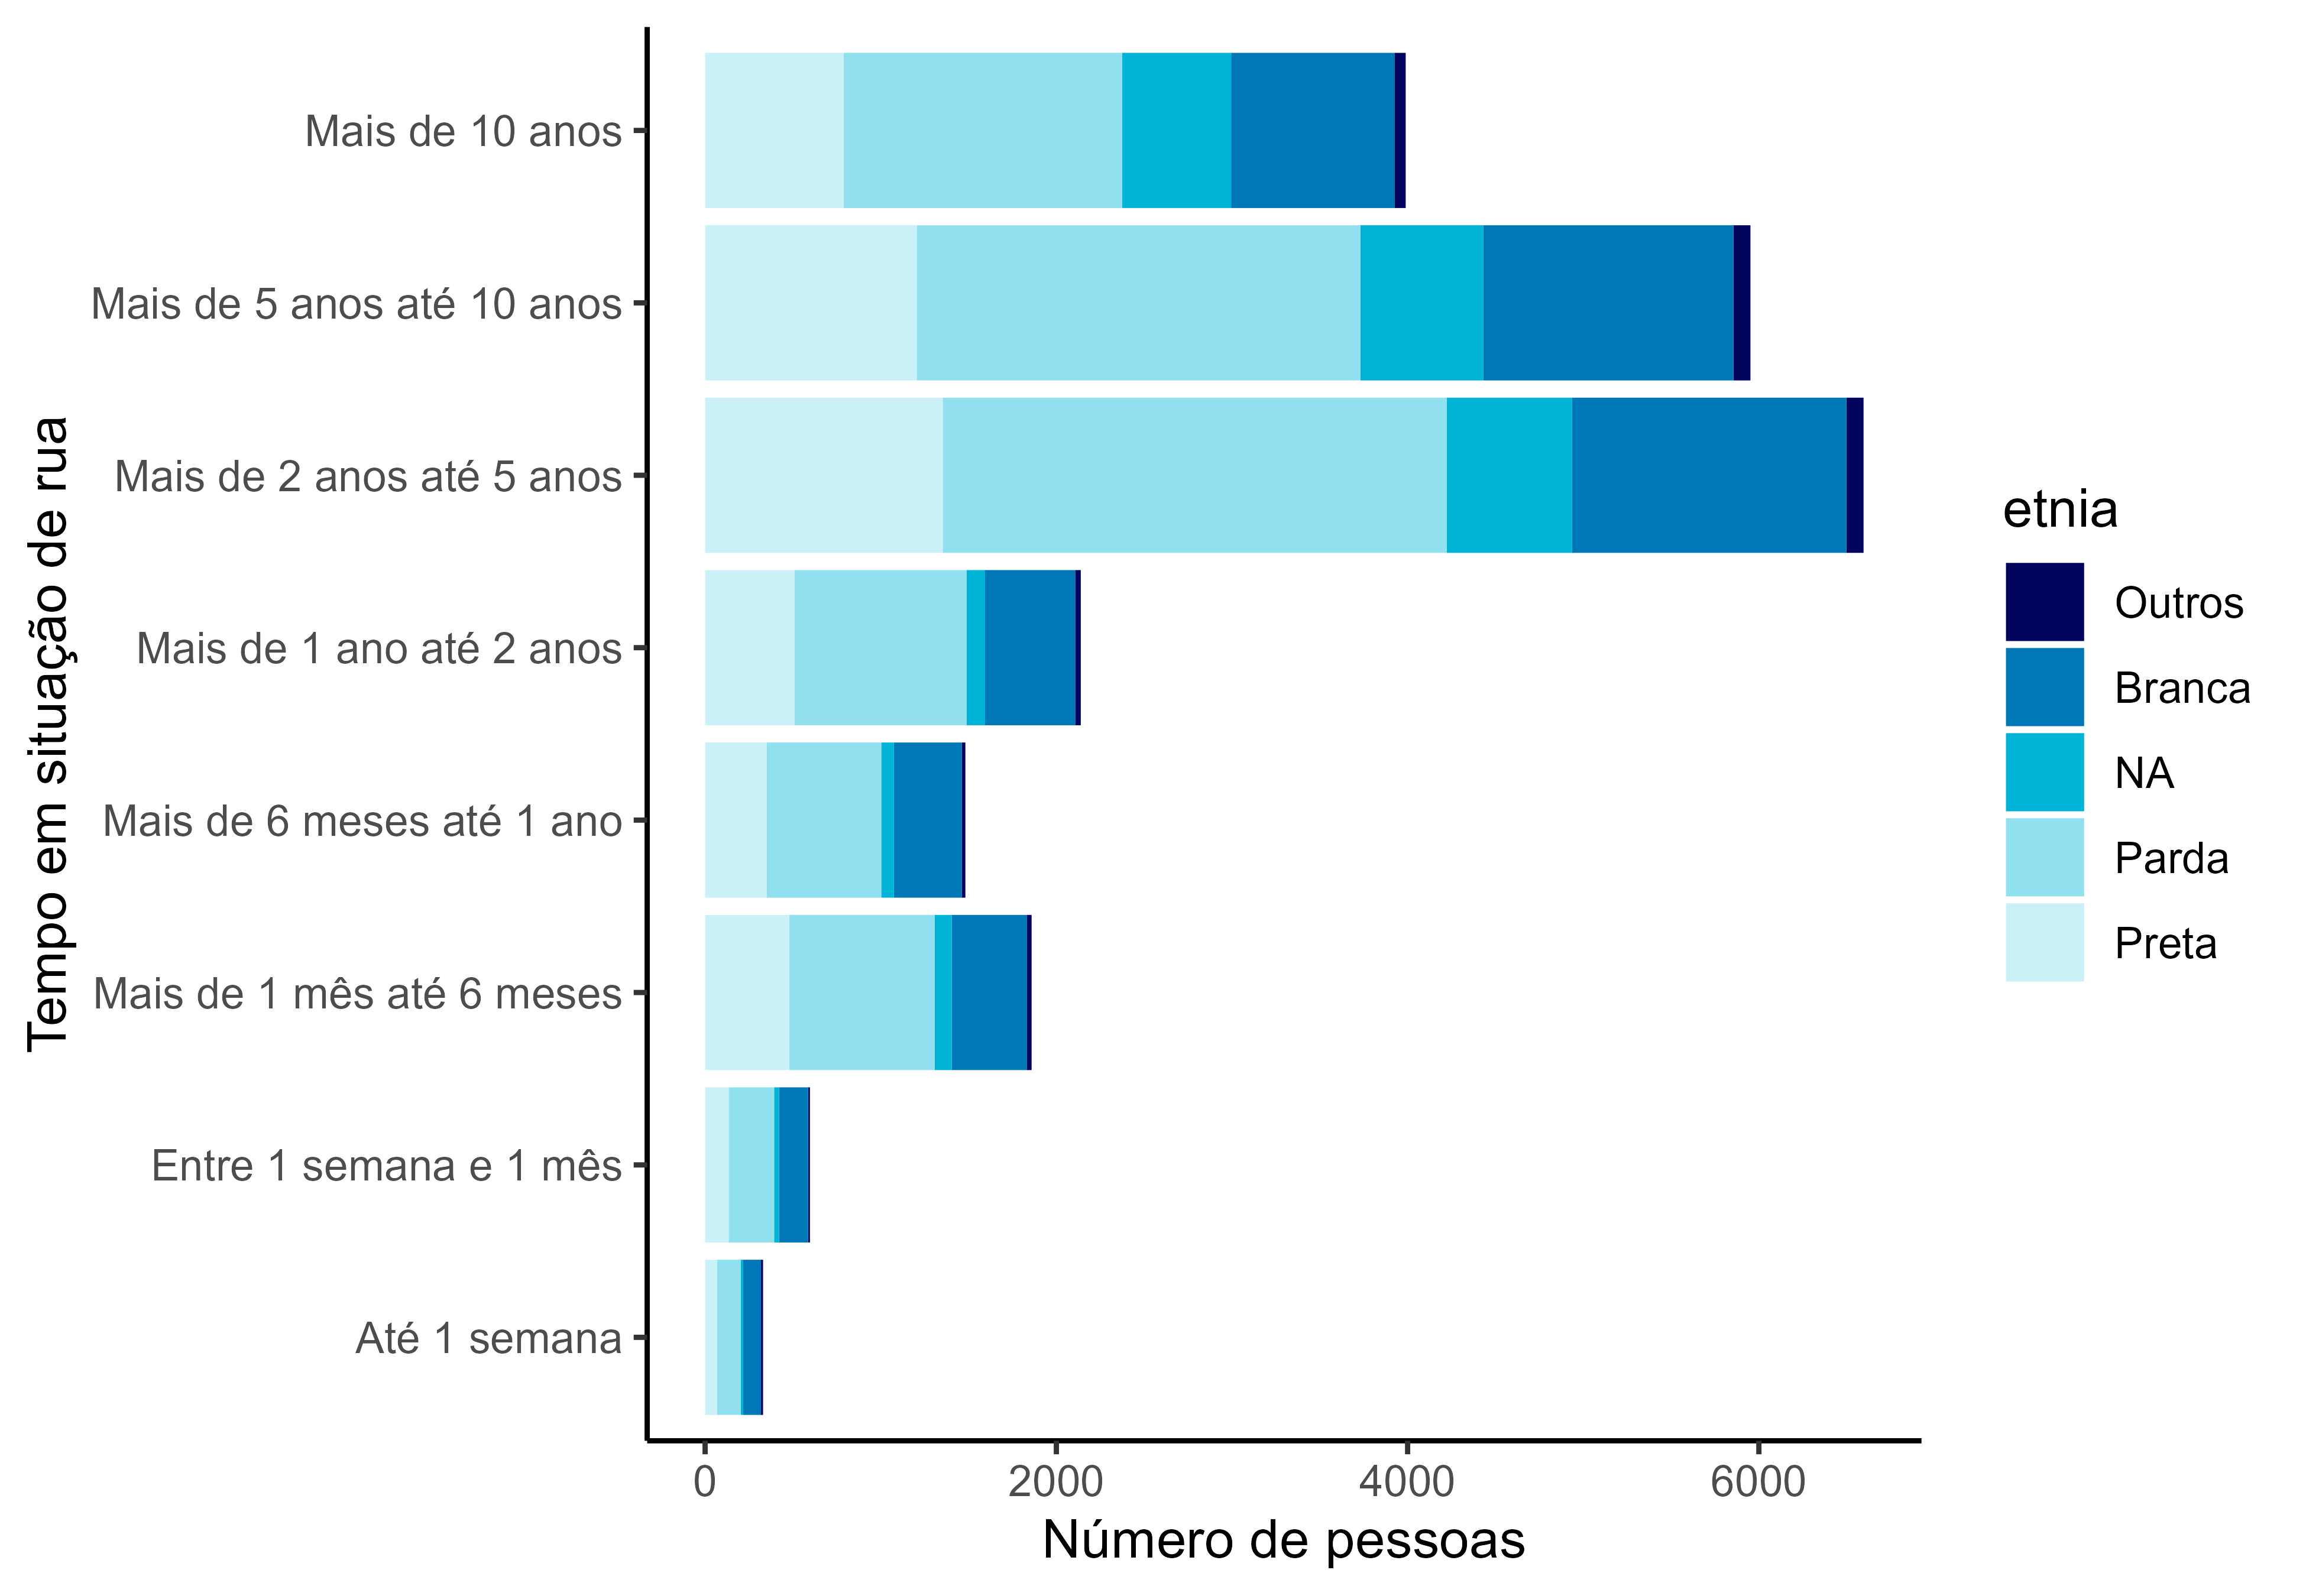
\includegraphics[width = .9\linewidth]{relatorios/grupo2/figuras/tempoderuaporetnia.png}
    \label{fig:tempoderuaetnia}
\end{figure}

\begin{figure}[h]
    \centering
    \caption{Evolução do RMA Anual por Centro POP}
    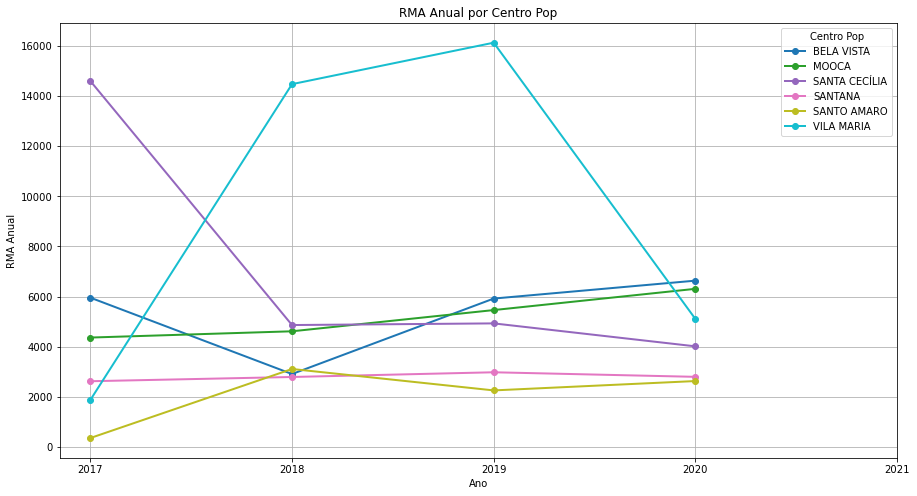
\includegraphics[width = .9\linewidth]{relatorios/grupo2/figuras/rma.png}
    \label{fig:rma}
\end{figure}

\begin{figure}[h]
    \centering
    \caption{Evolução do número de profissionais por função ao longo dos anos}
    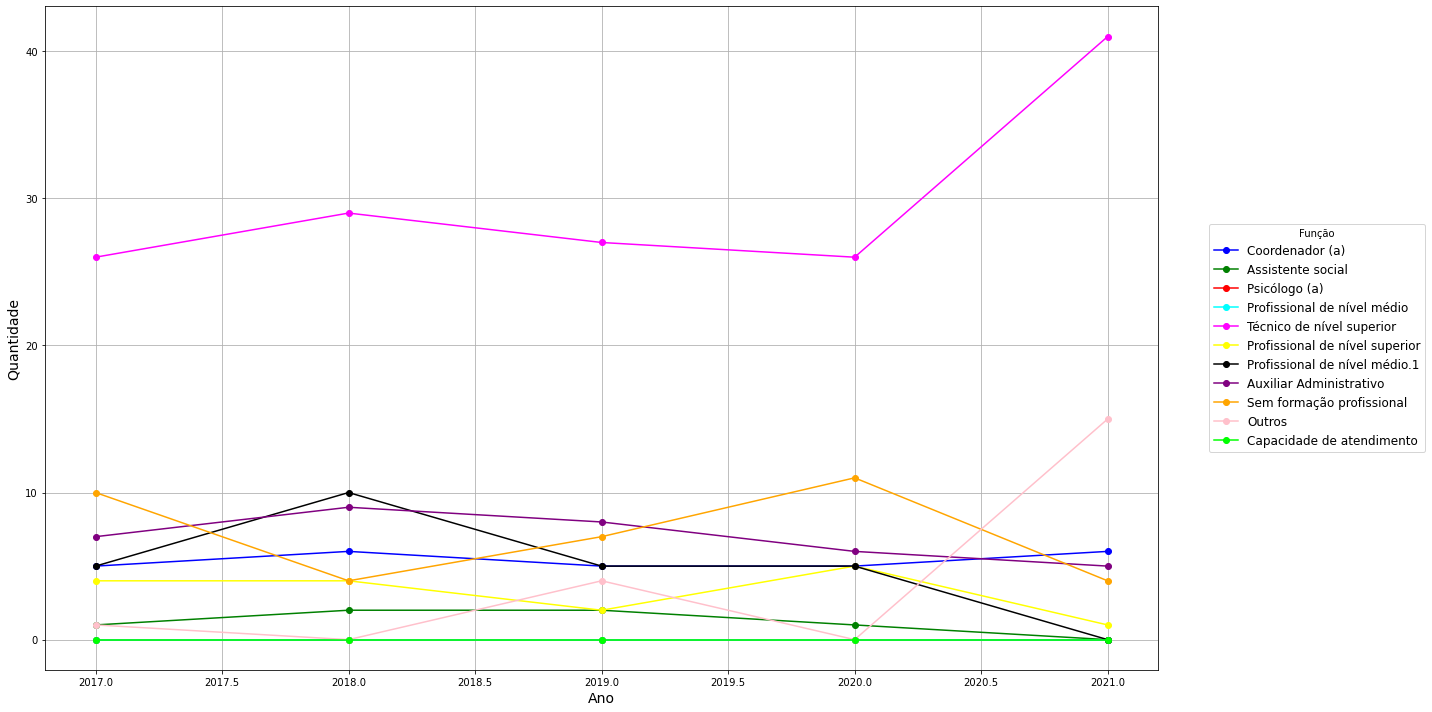
\includegraphics[width = .9\linewidth]{relatorios/grupo2/figuras/prof.png}
    \label{fig:prof}
\end{figure}



% \cite{natalino2016estimativa}
% \textcite{natalino2016estimativa}